\documentclass[tikz]{standalone}

\usepackage[utf8]{inputenc}
\usepackage[T1]{fontenc}
\usepackage{helvet}
\usepackage{../../templates/msc}

\renewcommand{\familydefault}{\sfdefault}

\tikzset{
every picture/.style={
line width=1pt
}}

\usepackage{tikz}
\author{Holger Karl}
\date{\today}
\title{}

\usetikzlibrary{calc}

\begin{document}

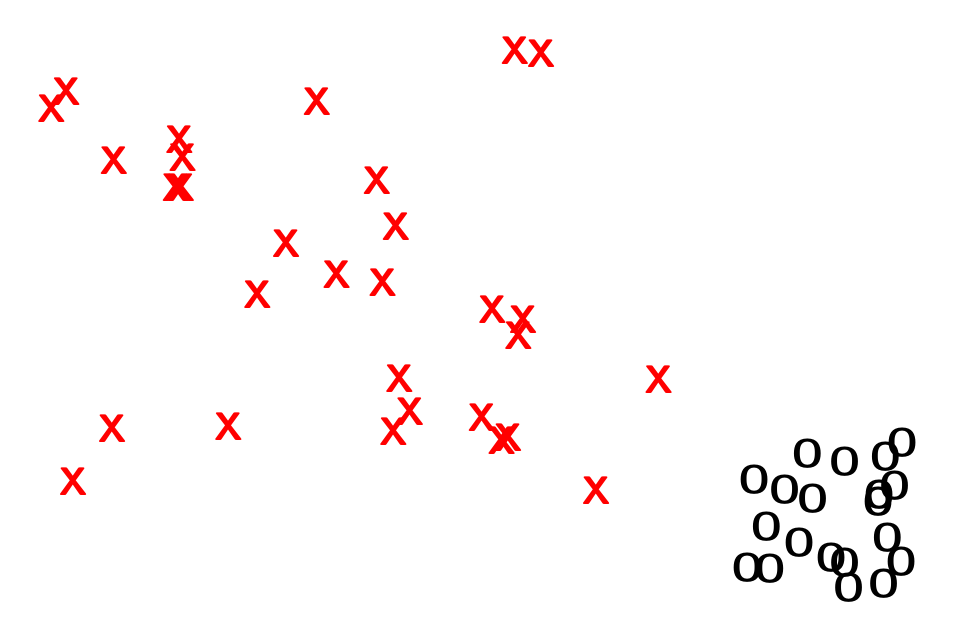
\begin{tikzpicture}
  \foreach \x in {1,2,...,30}{
    \node[text=red] at (4*rand+1, 3*rand+4) {\Large \textbf X}; 
  }
  \foreach \x in {1,2,...,20}{
    \node[text=black] at (1*rand+7, 1*rand+1) {\Large \textbf O}; 
  }
\end{tikzpicture}


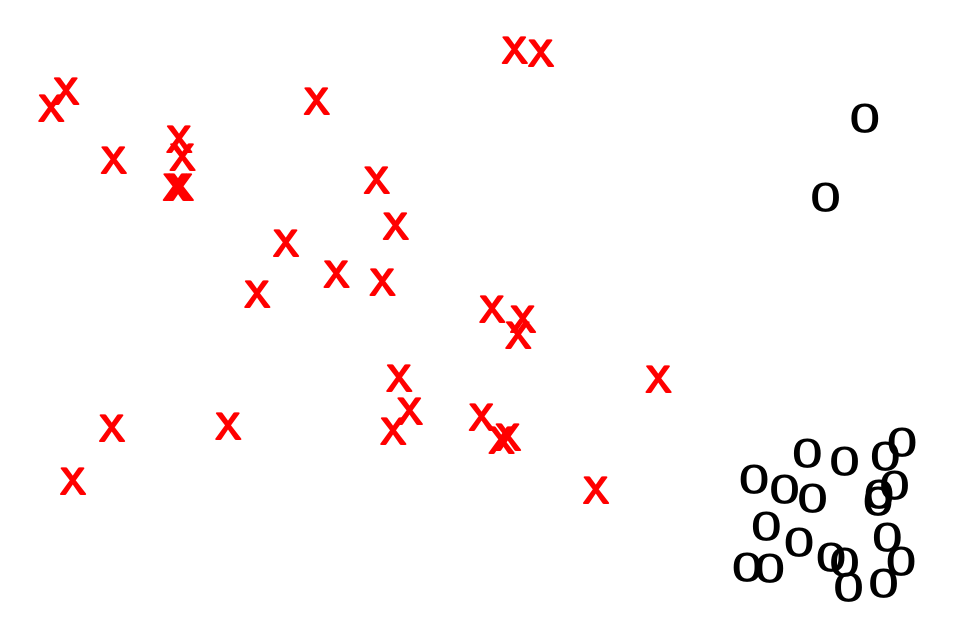
\begin{tikzpicture}
  \foreach \x in {1,2,...,30}{
    \node[text=red] at (4*rand+1, 3*rand+4) {\Large \textbf X}; 
  }
  \foreach \x in {1,2,...,20}{
    \node[text=black] at (1*rand+7, 1*rand+1) {\Large \textbf O}; 
  }

  \node[text=black] at (7,5) {\Large \textbf O}; 
  \node[text=black] at (7.5,6) {\Large \textbf O}; 
\end{tikzpicture}


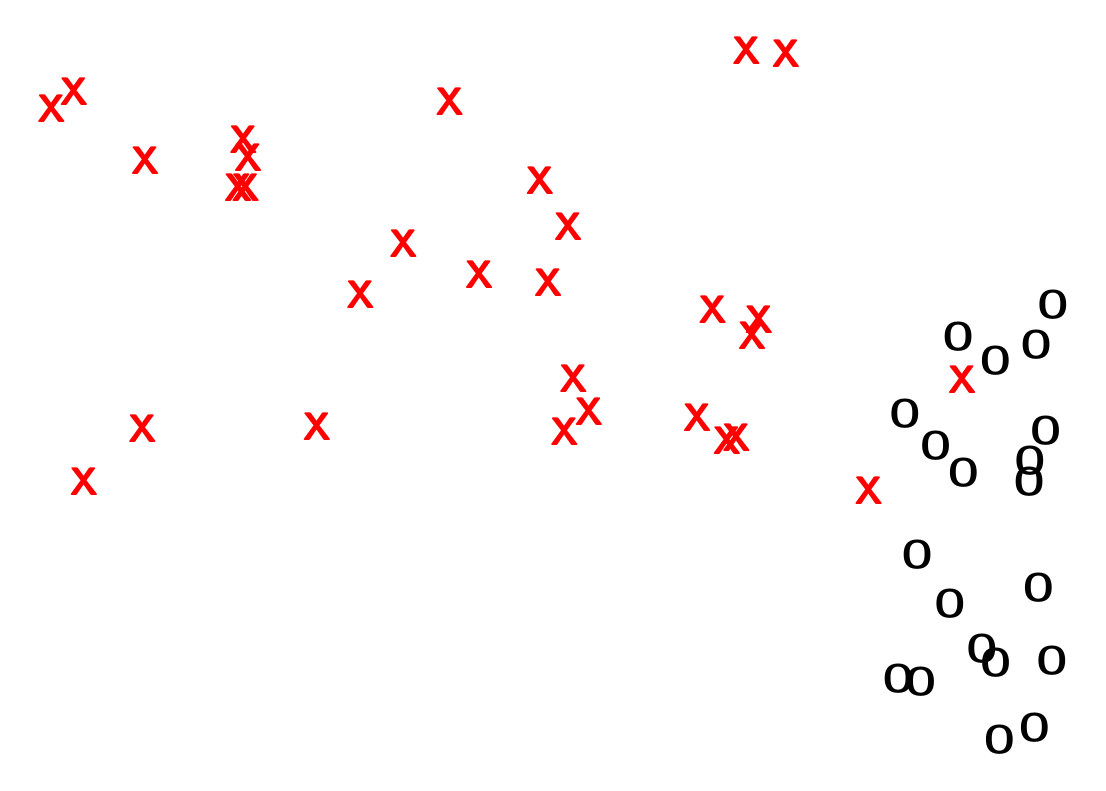
\begin{tikzpicture}
  \foreach \x in {1,2,...,30}{
    \node[text=red] at (6*rand+1, 3*rand+4) {\Large \textbf X}; 
  }
  \foreach \x in {1,2,...,20}{
    \node[text=black] at (1*rand+7, 3*rand+1) {\Large \textbf O}; 
  }
\end{tikzpicture}

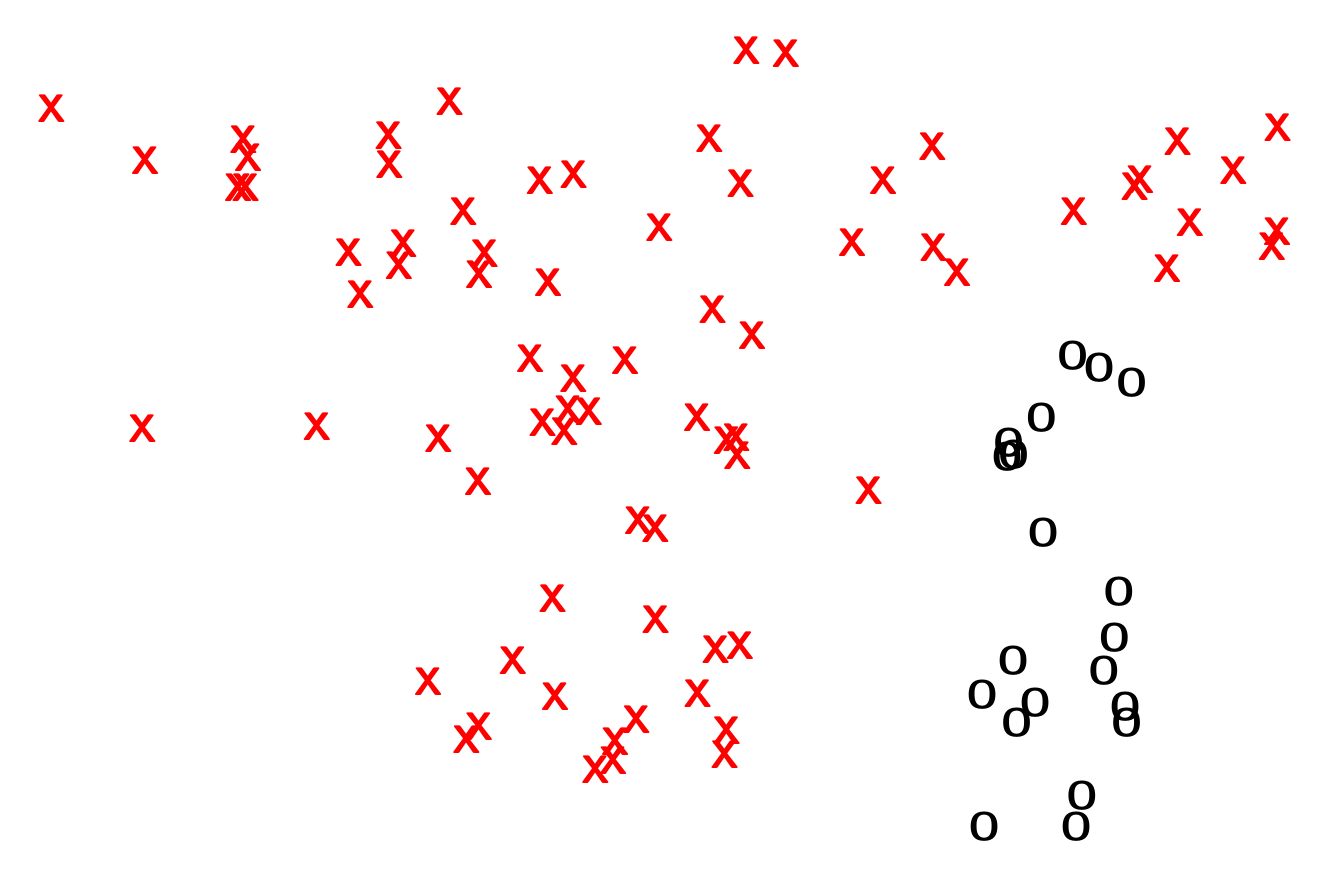
\begin{tikzpicture}
  \foreach \x in {1,2,...,25}{
    \node[text=red] at (6*rand+1, 3*rand+4) {\Large \textbf X}; 
  }
  \foreach \x in {1,2,...,25}{
    \node[text=red] at (6*rand+5, 1*rand+5) {\Large \textbf X}; 
  }
  \foreach \x in {1,2,...,25}{
    \node[text=red] at (2*rand+2, 3*rand+0) {\Large \textbf X}; 
  }

  \foreach \x in {1,2,...,20}{
    \node[text=black] at (1*rand+8, 3*rand+0) {\Large \textbf O}; 
  }
\end{tikzpicture}


\end{document}